%
% File: chap04.tex
% Author: Henry Semenenko
% Description: Chip-based MDI-QKD
%
% Set the graphics path to find figures
\graphicspath{{./chapters/chapter04/fig04/}}

\let\textcircled=\pgftextcircled
\chapter[Chip-Based Measurement-Device-Independent QKD]{Chip-Based Measurement-Device-Independent Quantum Key Distribution}
\label{chap:mdiqkd}

\section*{Statement of Work}

Again, this chapter made used of devices conceived and design by Mark Thompson and Mark Godfrey that were fabricated by Oclaro. The experimental setup was modified from the previous chapter with support from Philip Sibson. FPGA and RF electronic design was supported by Andy Hart. 

\section{Introduction}

Quantum technologies promise a paradigm shift compared to their classical counterparts that will undermine our current methods of secure communication \cite{shor1994}. It will soon become necessary to deploy key exchange systems that are immune to such increases in computing power. \ac{QKD} is one such approach which exploits quantum phenomena to exchange secret keys between distant parties without relying on assumed computationally hard problems \cite{BB84, E91}. However, the stringent requirements for precise control has predominately limited \ac{QKD} systems to small networks and laboratories. To realise ubiquitous quantum devices, new platforms are required for robust operation in harsh environments. 

Integrated photonics has seen vast improvements in recent years and represents a promising platform for mass-adoption of quantum technologies \cite{thompson2011}. In particular, \ac{InP} offers crucial benefits for communication in a robust, phase-stable and compact platform. Lasers can be monolithically integrated with mW powers and narrow linewidths, fast electro-optic phase modulation can reach bandwidths of \SI{40}{GHz} and low-loss waveguides allow efficient routing \cite{smit2014}. Such components mean that it is well suited for quantum communication protocols \cite{Sibson2017InP}. 

\Acl{QKD} has been a leading quantum technology since its advent \cite{BB84, E91} and has seen many proof-of-principle demonstrations, networks and commercial systems \cite{yin2016, Rubenok2013, Comandar2016, zhang2018, commercial}. However, implementation security of these systems is an active area of research due to potential information leakage that is not considered in security proofs. Such side-channels may allow an eavesdropper to gain sensitive information during a key exchange \cite{Lo2014} or an attacker to manipulate a system and determine the secret key through classical means \cite{Lydersen2010b}. 

To counter these attacks from a malicious adversary through uncharacterised side-channels, device-independent \ac{QKD} schemes have been developed to limit the number of assumptions required for security \cite{Masanes2011}. One such vulnerability is with single-photon detectors, for which \ac{MDI} has been proposed. This approach removes all possible attacks against the detection system \cite{mdi-qkd}.

In this section, we experimentally demonstrate \ac{MDI} using cost-effective, mass-manufacturable, chip-based transmitters that could facilitate commercial quantum-secured communication. We show that\SI{1}{kbps} of secret key can be exchanged at  \SI{100}{km} and predict positive key rates at more than \SI{350}{km}. The system removes detector vulnerabilities and represents a viable solution for near-term metropolitan quantum networks.

%Advances in \ac{QKD} have seen many protocols developed for different purposes and security levels. The emerging quantum hacking community has exposed discrepancies between security theory and practical implementations. 

%Technological advances require scalability. All currently available commercial \ac{QKD} systems are big, bulky and fibre-based. To encourage widespread adoption beyond commercial and military applications, an integrated platform it required to require manufacturing costs, as well as the size, weight and power requirements. \ac{QKD} transmitters have been demonstrated in both \ac{InP} \cite{Sibson2017InP} and silicon \cite{Sibson2017Si}.

%In this section, we will be experimentally demonstrating \ac{MDI} \cite{mdi-qkd} using integrated \ac{InP} transmitter devices. We will first outline the \ac{MDI} protocol before describing the experiment and showing our results. We will then discuss potential improvements to the experiment and further work.

%=======
\section{Measurement-Device-Independent Quantum Key Distribution}
\label{sec:mdi-qkd}

\Ac{MDI} removes all potential side channels on the detection system which could be exploited by a malicious adversary \cite{mdi-qkd}. A schematic of the experiment is shown in figure~\ref{fig:chip-mdi}. Unlike traditional point-to-point protocols, Alice and Bob act symmetrically by sending BB84 states to a third party, Charlie. Upon receipt of the states, Charlie measures the states in the Bell basis and publicly announces all successful events. The outcomes indicate quantum correlations between states but, without encoding knowledge known only by Alice and Bob, reveal no information about the secret key. This allows Charlie to be completely untrusted and it could even be assumed that an adversary is operating the receiver without compromising the security. By sharing the basis information for each state, Alice and Bob are able to infer a secret key which can be used in a symmetric key algorithm. 

As we use a weak coherent source we need to estimate the number of single-photon events. We employ a four-intensity decoy state analysis \cite{zhou2016} to bound the single-photon errors and yields. In this protocol, the $Z$ basis is used to generate key while the $X$ basis bounds the knowledge of an eavesdropper. 

While\Ac{MDI} typically offers a lower key rate at short distances when compared with point-to-point systems \cite{Sibson2017InP}, it can generate key rate at greater distances \cite{yin2016} as the errors are proportional to the square of the dark count probability. It also offers the potential for the measurement equipment to be shared between multiple parties through optical switching without compromising security.

Unlike a traditional point-to-point key exchange, \ac{MDI} introduces third party (Charlie) who mediates the exchange by announcing correlations between pulses sent by Alice and Bob. Importantly, the scheme removes unnecessary assumptions about the characteristics of the detection system meaning that 

it improves security by removing all, current and future, side-channels on the detectors \cite{mdi-qkd}. This is an important step as the detectors are often vulnerable to attacks due to their complexity \cite{Lydersen2010a, Makarov2006}. In this case, it doesn't need to be assumed that Charlie is a trusted party and the node could equally be operated by Eve or Mallory. Any interference at the detections by a malicious attacker will only reduce the possible key rate, so is equivalent to a denial of service attack.

Secondly, it removes the asymmetry between Alice and Bob which allows for simpler metropolitan networks without reducing security with trusted nodes. This will be discussed further in chapter \ref{chap:node}.

\subsection{Protocol}

\begin{figure}[tbp]
	\centering
	\includegraphics[scale=0.25]{MDI-QKD_Protocol.png}
	\caption[MDI-QKD protocol]{Measurement-device-independent quantum key distribution protocol schematic for time-bin encoding. Alice and Bob act symmetrically by sending BB84 states to a third party, Charlie, who projects the states in the Bell basis. Charlie announces all successful events from which Alice and Bob can infer a key after sharing state basis information.}
	\label{fig:mdi_protocol}
\end{figure}

An outline of the protocol is shown in figure \ref{fig:mdi_protocol}. We will use a four decoy state protocol \cite{zhou2016} which treats the $Z$ and $X$ bases separately. The $Z$ basis is used entirely to generate keys, while the $X$ basis is used to bound knowledge gained by an eavesdropper. This is optimal for the symmetric case. The asymmetric case needs to be dealt with slightly differently \cite{wang2018}.

\begin{enumerate}
	\item \brisred{Preparation} Alice and Bob independently and randomly choose \acp{wcs} from the BB84 states. 
	\item \brisred{Measurement} Charlie performs joint Bell state projections on states from Alice and Bob
	\item \brisred{Announcement} Each successful projection is publicly announced by Charlie, along with timing information.
	\item \brisred{Basis Discussion} Alice and Bob each announced the basis chosen for each successful projection.
	\item \brisred{Parameter Estimation} Using the information about successful events, they can calculate errors and gains to bound the knowledge of Eve and apply privacy amplification if necessary.
\end{enumerate}

\begin{table}[tbp]
\centering
\begin{tabular}{@{}cccc@{}}
\textbf{Basis}      & $\ket{\psi^-}$     & $\ket{\psi^+}$        \\
$Z$              & Bit flip           & Bit flip                \\
$X$              & Bit flip           & \multicolumn{1}{c}{-}   \\
\end{tabular}
\caption[Measurement outcomes in MDI-QKD]{Post-selection rules of measurement outcomes in different bases. If Alice and Bob sent states in the same basis, one of them will have to bit-flip unless the both chose the X basis and the result was $\ket{\psi^+}$.}
\label{tab:mdi-outcomes}
\end{table}

\subsection{Security and Key Rates}

As we are not using a true single photon source, we need to be able to bound any knowledge gained by Eve through a photon number splitting attack. This is done through decoy-state analysis, where various intensity levels are chosen at random to bound the yield and error for single photon states \cite{Lo2005}. 

Here we used a four intensity decoy state protocol where we consider four sources: $\nu, \sigma, \mu, z$. The $\nu$ source is vacuum, $\sigma$ and $\mu$ are decoy pulses in the $X$ basis with average photon numbers $\sigma$ and $\mu$, respectively. Finally, the $z$ source emits pulses with intensity $z$ in the $Z$ basis. In an \ac{MDI} protocol, we use the $X$ basis to bound the knowledge of Eve or Mallory and the $Z$ basis to generate key. This is due to the minimum possible error of $25\%$ in the $X$ basis \cite{Rubenok2013}.

The estimate key rate of \ac{MDI} per pulse in the infinite case is given as

\begin{equation}
	R = (p_z)^2 Y_{11}^Z \left(1 - H_2(E_{11}^X)\right) - Q_{s,s}^Z f_e E_{S,S}^Z H_2(E_{\mu_s\mu_s}^Z)
\end{equation}
where $Y_{11}^Z$ and $e_{11}^X$ are the yield in the $Z$ basis and error in the $X$ basis, respectively, when Alice and Bob both sent single photons. These quantities are not directly measurable so we will need to bound them using a decoy state protocol. $Q_{S,S}^Z$ and $E_{S,S}^Z$ are the gain and error in the $Z$ basis and both can be measured directly. Finally, we introduce the error correction efficiency, $f_e>1$, and the binary entropy function defined as
\begin{equation}
	H_2(x) = -x\mathrm{log}_2(x) - (1-x)\mathrm{log}_2(1-x).
\end{equation}

As we are not using single photons, we cannot determine the single photo errors and yields exactly. Therefore, we need to use a decoy state technique \cite{Lo2005} to give lower and upper bounds of $Y_{11}^Z$ and $E_{11}^X$, respectively. We then need to define the lower bound of the secret key rate as
\begin{equation}
	\underline{R} \geq R
\end{equation}
In essence, decoys states are measuring the loss of the channel during a key exchange to bound the knowledge that could be gain by an eavesdropper.  By measuring different intensities in a decoy state protocol, we can measure

\begin{equation}
	Q_{\mu_a \mu_b}^Z = \sum_{n,m=0} e^{-(\mu_a + \mu_b)}\frac{\mu_a^n}{n!}\frac{\mu_b^m}{m!} Y_{n,m}^Z
\end{equation}

\begin{equation}
	Q_{\mu_{a} \mu_{b}}^X E^{X}_{\mu_{a} \mu_{b}}=\sum_{n, m=0} e^{-\left(\mu_{\mathrm{a}}+\mu_{\mathrm{b}}\right)} \frac{q_{\mathrm{a}}^{n}}{n !} \frac{q_{\mathrm{b}}^{m}}{m !} Y^{X}_{n, m} E^{X}_{n, m}
\end{equation}
where $\mu_a$ ($\mu_b$) are the intensities of Alice's (Bob's) pulses. The gain, $Q_{\mu\sigma}^i$, defined to be the number of successful Bell state projections when Alice and Bob send states in the basis $i$ with intensities $\mu$ and $\sigma$ respectively.

\begin{equation}
	\underline{Y_{11}^Z} = \frac{1}{\left(\mu_{\mathrm{a}}-\omega_{\mathrm{a}}\right)\left(\mu_{\mathrm{b}}-\omega_{\mathrm{b}}\right)\left(v_{\mathrm{a}}-\omega_{\mathrm{a}}\right)\left(\nu_{\mathrm{b}}-\omega_{\mathrm{b}}\right)\left(\mu_{\mathrm{a}}-v_{\mathrm{a}}\right)}
\end{equation}

\begin{equation}
	\overline{E_{11}^Z} = \frac{1}{\left(v_{\mathrm{a}}-\omega_{\mathrm{a}}\right)\left(v_{\mathrm{b}}-\omega_{\mathrm{b}}\right) \underline{Y^{X}_{1,1}}}
\end{equation}

In the infinite case, $Y_{11}^Z = Y_{11}^X$ so we can use the decoy sates in $X$ to bound the single photon events in $Z$ \cite{zhou2016}. 

\subsection{Model}

\begin{figure}[tbp]
\begin{tikzpicture}
\begin{semilogyaxis}[
    axis line on top,
	xlabel = {Error (\%)},
	ylabel = {Secret Key Rate (bps)},
	width = 0.9\linewidth,
	height = 0.5\linewidth,
	cycle list name = RdYlPu-8,
	xmin = 0,
	xmax = 1.8,
	xtick pos=left,
	ytick pos=left,
    tick align=outside,
    grid=both,
    grid style={line width=.1pt, draw=gray!10},
    legend style={fill=blue!5, draw=gray!50}
	]
\foreach \y in {1,...,8}{
  \addplot+[very thick] table[x index=0,y index=\y, col sep=comma] {./chapters/chapter04/fig04/error_skr.csv};
  \temp
}
\legend{\SI{0}{\km},\SI{50}{\km},\SI{100}{\km},\SI{150}{\km},\SI{200}{\km},\SI{250}{\km},\SI{300}{\km},\SI{350}{\km},}
\end{semilogyaxis}
\end{tikzpicture}
	\caption[Error dependence of secret key rate]{By varying the error rate in the signal $Z$ basis, while maintaining consistent errors in the $X$ basis, we can see the dependence of the quantum bit errors. As the $Z$ basis is used only to generate key, the error must be kept low, especially at longer distances.}
	\label{fig:skr_error_dependence}
\end{figure}

From the parameters of the system (photon numbers and errors), we can create a model to verify that the system behaves as expected. This will also allow us to predict the performance of the system at further distances without needing to gather data for days or weeks. 

The detectors used in this system are \acp{snspd} due to their high efficiency and low dead-time and jitter \cite{}. The detectors operate at $80\%$ efficiency, with a dead-time of \SI{<100}{ns} and jitter of \SI{30}{ps}. The average photon number per state is calibrated before a key exchange by estimating the losses through the system and detection efficiency.

The gain of the system, $Q^{ \{X,Z\} }$, is the probability of projection onto a Bell state in either the $X$ or $Z$ basis. We can estimate the gain from the average photon number of each transmitter, the detection efficiency and the transmitters loss. We will assume that the transmission loss is the standard \SI{0.2}{dB/km}, although fibre optic losses can be as a low as \SI{0.17}{dB\per\km} \cite{corningULL}. The gain is independent of error, so we can estimate the gain as 

\begin{equation}
	Q^{ \{X,Z\} } = \frac{3}{8}  \times \eta^2 \times \left( 1 - \text{exp} \left( -10^{- \frac{0.2 \times L}{2 \times 10} \mu}  \right)  \right)^2 + Q^{d.c.}
\end{equation}
where $Q^{d.c.}$ are the successful projections that are because of dark counts in the system. As \acp{snspd} have dark counts of \SI{100}{Hz} this value is typically $\left(10^{-6}\right)^2$. The value is quoted as squared as we are looking for coincidences between the two detectors. 

The prefactor of \nicefrac{3}{8} is due to the probability of a successful projection give two random states sent by Alice and Bob. On half of the time, the states will be projected onto a Bell state that cannot be determined by the measurement device \cite{}. Of the remainder, one half will be projected successfully onto $\ket{\psi^-}$ (\nicefrac{1}{4} of the total states), while with probability \nicefrac{1}{2} they will be successfully projected onto $\ket{\psi^+}$ (\nicefrac{1}{8} of the total states). 

To calculate the probability of coincidence from the coherent states, we take the (slight) simplification of one minus the probability of zero photons multiplied by the detection efficiency, $\eta$. While the true probability will vary due to multiphoton terms, the amplitude of the coherent states is sufficiently low ($\le 0.2$ at \SI{0}{\km}) the multiphoton terms will not play a large role, especially at longer distances. The attenuation on each state is calculated, assuming \SI{0.2}{dB\per\km}, a the distance between Alice and Bob, $L$, is halved as Charlie sits at a location halfway between them.

To model the errors, we need to include contributions from dark counts in the system.

\begin{equation}
	E^{\{X,Z\}}_{m,n} = \frac{\left(Q^{\{X,Z\}}_{m,n} - Q^{d.c}\right) \times \epsilon + Q^{d.c} \times 0.5}{Q^{\{X,Z\}}_{m,n}}
\end{equation}



\subsection{Shared Resources}

As \ac{MDI} introduces Charlie to mediate the key exchange, this easily facilitates sharing resources by switching between users connecting to a centralised node. In a metropolitan network, each used can access the quantum network with a transmitter device and through simple switching allows all users to exchange secret keys with every other user. Such optical switches are already available commercially with less than \SI{1}{dB} insertion loss which is acceptable for \ac{QKD} system \cite{polatis}. While superconducting detectors are generally considered a piece of research equipment, there have been many advances in the technology of both the detector fabrication to cryogenic coolers which meant that widespread usage on \acp{snspd} should be anticipated. More advanced quantum networks will be heavily dependant on the unrivalled specifications that \acp{snspd} offer.

\section{Integrated Transmitters}

The \ac{InP} transmitters provide all the required components to create high fidelity BB84 states that are required for \ac{MDI}. By using chip-based transmitters the power, size and weight of the optics needed can be dramatically reduced compared to fibre (and free-space) alternatives. It also facilitates mass production without requiring manual assembly. 

It is worth noting that the technology is still maturing and optimisation of designs is still required before devices can be confidently reproduced to a required standard for secure communication. The transmitters used for this experiment (figure \ref{fig:oclaro_00}) were originally designed to operate as transceiver\footnote{A device which is capable of transmitting the quantum signal as well as receiving it.} which would allow two-way operation. However, the delay line was found to be too lossy to be useful, showing how further optimisation of designs is required.

In this section, we will describe the operation of the transmitters to create weak coherent states that can be used for \acl{QKD}.

\begin{figure}[tbp]
\centering
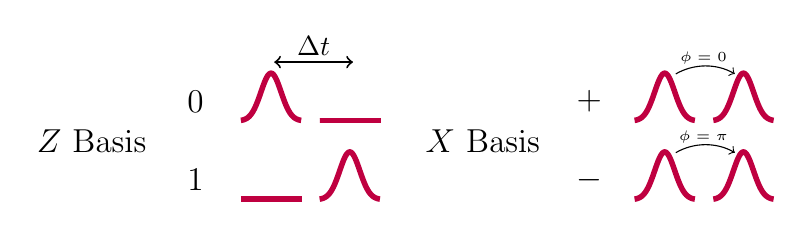
\begin{tikzpicture}
%%X basis
\node[left] at (-0.5, 3.8) {\large $X$ Basis};
%%+
\node[] at (0,4.3) {\large $\ket{+}$};
\begin{axis}[xshift = 0.5cm,yshift=4cm,axis lines=none,width=2.5cm, height = 2.3cm]
\addplot[
purple,
domain=-3:3,
samples=201,
line width=2pt
]
{exp(-x^2 / 2) / (1* sqrt(2*pi))};
\end{axis}
\draw[->] (1.1,4.65) arc (120:60:0.75);
\node[] at (1.45,4.85) {\tiny $\phi = 0$};
\begin{axis}[xshift = 1.5cm,yshift=4cm,axis lines=none,width=2.5cm, height = 2.3cm]
\addplot[
purple,
domain=-3:3,
samples=201,
line width=2pt
]
{exp(-x^2 / 2) / (1* sqrt(2*pi))};
\end{axis}
%%-
\node[] at (0,3.3) {\large $\ket{-}$};
\begin{axis}[xshift = 0.5cm,yshift=3cm,axis lines=none,width=2.5cm, height = 2.3cm]
\addplot[
purple,
domain=-3:3,
samples=201,
line width=2pt
]
{exp(-x^2 / 2) / (1* sqrt(2*pi))};
\end{axis}
\draw[->] (1.1,3.65) arc (120:60:0.75);
\node[] at (1.45,3.85) {\tiny $\phi = \pi$};
\begin{axis}[xshift = 1.5cm,yshift=3cm,axis lines=none,width=2.5cm, height = 2.3cm]
\addplot[
purple,
domain=-3:3,
samples=201,
line width=2pt
]
{exp(-x^2 / 2) / (1* sqrt(2*pi))};
\end{axis}
%%Z basis
\node[left] at (-5.5, 3.8) {\large $Z$ Basis};
%%+0
\node[] at (-5,4.3) {\large $\ket{0}$};
\begin{axis}[xshift = -4.5cm,yshift=4cm,axis lines=none,width=2.5cm, height = 2.3cm]
\addplot[
purple,
domain=-3:3,
samples=201,
line width=2pt
]
{exp(-x^2 / 2) / (1* sqrt(2*pi))};
\end{axis}
\begin{axis}[xshift = -3.5cm,yshift=3.7cm,axis lines=none,width=2.5cm, height = 2.3cm]
\addplot[
purple,
domain=-3:3,
samples=201,
line width=2pt
]
{0};
\end{axis}
%%1
\node[] at (-5,3.3) {\large $\ket{1}$};
\begin{axis}[xshift = -4.5cm,yshift=2.7cm,axis lines=none,width=2.5cm, height = 2.3cm]
\addplot[
purple,
domain=-3:3,
samples=201,
line width=2pt
]
{0};
\end{axis}
\begin{axis}[xshift = -3.5cm,yshift=3cm,axis lines=none,width=2.5cm, height = 2.3cm]
\addplot[
purple,
domain=-3:3,
samples=201,
line width=2pt
]
{exp(-x^2 / 2) / (1* sqrt(2*pi))};
\end{axis}
\draw[<->, line width = 0.25mm] (-4,4.8) -- (-3,4.8);
\node[] at (-3.5,5) {$\Delta t$};
\end{tikzpicture}
\caption[BB84 time-bin encoding]{BB84 states in a time-bin encoded scheme. Pulses are separated by a time $\Delta t$ where the timing forms the computational basis. A late pulse indicates a $\ket{0}$ while an early pulse indicates a $\ket{1}$. $\ket{+}$ and $\ket{-}$ states can be realised through superpositions of early and late pulses with relative phases.}
\label{fig:BB84_time_bin}
\end{figure}

\begin{figure}[tbp]
	\centering
	\includegraphics[width=\textwidth]{Oclaro_00_clean_small.png}
	\caption[InP transmitter microscope image]{Microscope image of the \SI[product-units=power]{6x2}{mm} indium phosphide transmitter. The complexity possible with integrated photonics is demonstrated by having two separate DBR cavity lasers, three Mach-Zehnder interferometers, an asymmetric  Mach-Zehnder interferometer and high-bandwidth photodiode.}
	\label{fig:oclaro_00}
\end{figure}

\begin{figure}[tbp]
	\includegraphics[width=\linewidth]{Oclaro_00_MDI.png}
	\caption[InP transmitter schematic]{A schematic view of the each chip used in the MDI-QKD protocol. \textit{T. Enc} is used to intensity modulate the continuous wave laser into encode timing information, \textit{I. Mod} varies the pulse intensity for decoy state preparation and \textit{Ph. Enc} encodes phases between the time-bins.}
	\label{fig:chip_mdi_schematic}
\end{figure}

\subsection{Pulse Carving}

As for the previous chapter, time encoding the states will be done using a \acl{mzi} to carve the \ac{CW} laser into \SI{130}{ps} pulses with an extinction ratio\footnote{The ratio between the ``on'' and ``off'' powers of the \ac{mzi}} of up to \SI{30}{dB}.

To encode a state in the diagonal basis, the \ac{mzi} carves two pulses in quick succession. This requires that the coherence length of the laser is longer than the pulse separation to ensure coherence within a state. 

\subsection{Phase Encoding}

Also using an \ac{mzi}, phase can be encoding through a "push-pull" method. By either pulsing the top or bottom \ac{eopm}, a relative $\pi$ phase can be imparted on pulses.

\subsection{Phase Randomisation}

A negative pulse can be used to gain switch the on-chip laser in between states to randomise the phase. 

\begin{figure}[tbp]
	\centering
	\def\svgwidth{\textwidth} 
	\import{chapters/chapter04/fig04/}{states.pdf_tex}
	\caption[BB84 states generated from the InP transmitters]{BB84 states generated from the InP transmitters using cascaded \acp{mzi}. They demonstrate a \SI{30}{dB} extinction ratio and a \SI{130}{\ps} \ac{FWHM} which includes broadening due to detector jitter.}
	\label{fig:states}
\end{figure}

\subsection{Decoy State Preparation}

While the absoption of the \ac{qcse} is an issue when encoding phase, it can be used to vary the intensity for decoy state preparation. The effect has a bandwidth of \SI{>10}{\GHz}. By biasing a modulator in the circuit to \SI{9}{\V} below the chip ground, we can quickly modulator with around \SI{2}{\Vpp} to vary the intensity by \SI{15}{dB}. We are also able to choose whether we pulse the intensity \ac{mzi} which creates the pulses which can be useful for encoding a vacuum state with an intensity of \SI{30}{dB} below that of signal states.

As the intensities of the decoy states is not fix, we will need to model how these intensities will vary the secret key rate. It has been previously shown that reducing the intensity of decoy states will increase the secret key rate \cite{Chan2014}. However, we will still 

\subsection{State Choice}

In a \ac{QKD} system, the states should be chosen randomly. However, for simplicity in this proof-of-principle experiment the states send by Alice and Bob are a fixed pattern chosen to gather statistics of all of the possible combination of states required for key rate estimation. States that play no part in key rate estimation (for example when Alice sends a state in $X$ and Bob in $Z$) are deliberately removed. In the asymptotic limit, sending these states would not impact the key rate. We will discuss later how these sorts of states would need to be considered in a finite key rate estimation.

\section{Control Electronics}

In order to operate the transmitters, there is a selection of control devices needed. In this section we will describe them.

For each transmitter, we require four RF signals with different requirements. For example, the decoy state analysis requires multiple levels while the phase randomisation only requires two levels, but needs to be very stable.

To synchronise the equipment, one AWG provided a clock that could be shared. The FPGA received a \SI{250}{\MHz} clock and each \ac{ppg} received a \SI{2}{\GHz} from the AWG. 

\begin{figure}[tbp]
	\centering
	\includegraphics[width=\textwidth]{experiment_control}
	\caption[Control electronic schematic of the MDI-QKD experiment]{The experiment required a number of pieces of equipment to control the transmitters and provide synchronisation signals for the detection. This figure shows the ``control plane'' of the experiment.}
	\label{fig04:exp_control}
\end{figure}

\subsubsection*{Temperature Control}

Two Arroyo 6301 are used to stabilise the temperature of each transmitter independently. A \SI{10}{K} thermistor is put into the base of the transmitter package as close as possible to the transmitter. Thermal paste is used to ensure a good thermal contact to the mount and the silver epoxy used for the chips provides a good thermal contact to the chip. A peltier is used to heat and cool the package through a thermo-electric effect and can be driven with up to \SI{3}{A} of current. The transmitters dissipate very little heat as most of the operation relies on electro-optic effects. Some heating is caused by thermo-optic modulation and laser driving. The temperatures are chosen to be above the ambient room temperature and to also to overlap the wavelengths between the two lasers. Typical temperatures we between \SI{25}{\celsius} and \SI{30}{\celsius}, required around \SI{100}{mA} from the Arroyo controller and had an instability of less than \SI{0.01}{\celsius}. Good temperature stability of the chips is important as much of the optical circuit is vert temperature sensitive. A change in temperature will cause the cavity to expand or contract to change the wavelength. It can also cause a change in the operating conditions of the \acp{mzi} due to phase differences in the top and bottom arms and  

\subsubsection*{Laser Driver}

The same Arroyo 6301 boxes also provided stable current sources to drive the on-chip lasers. The lasers show a threshold current of \SI{12}{mA} and can be driven with voltages above \SI{100}{mA}. As well as an increase in power, an increase in current will provide a wavelength shift due to heating in the cavity. With a current precision of \SI{0.01}{mA}, the wavelength of the laser can be controlled in steps of \SI{80}{fm} through heating and carrier effects in the \ac{SOA}. This provides the find control for high-fidelity overlap between independently operated transmitters. 

\subsubsection*{Modulator Biasing}

For the \ac{qcse}, a reverse bias over the modulator was required. Due to the lack of a negative voltage source, the ground of the chip was set to \SI{10}{V} from which lower biases could be set for the modulator to create a reverse bias.

Heating was also required. Up to \SI{120}{mA} was used to thermo-optically modulate the light in the \acp{mzi}.

\subsubsection*{Thermo-Optic modulation}

Ideally, the light in a \ac{mzi} would experience the same phase in both arms. However, due to fabrication tolerances, the light in each arm accumulates a different phase, meaning that the output is no longer minimised. While this could be corrected using the \ac{qcse}, the phase dependent loss mean that the extinction ratio would be reduced as the intensity of light would be different in each arm. Instead, we can exploit an imperfection in the \acp{eopm} which causes a resistance of around \SI{10}{\ohm}. By passing a current through the modulator on one arm of a \ac{mzi}, we can adjust the relative phase which will minimise the \ac{mzi} output intensity.

\subsubsection*{High-Speed Electronics}

A variety of high-speed driving electronics was used. Each transmitter requires four high-speed signals for phase randomisation, timing encoding, intensity modulation and phase encoding. Only the intensity modulation, which is used for the decoy state preparation, requires more than a two level signal. To create the signal and two decoy intensities, we will require a three level signal. 

\begin{figure}[tbp]
	\centering
	\def\svgwidth{0.9\textwidth} 
	\import{chapters/chapter04/fig04/Electrical_Signals/}{plot.pdf_tex}
	\caption[Electrical signals for BB84 states]{Oscilloscope data of the electrical signals required for the BB84 states. P. Mod is used to create the pulses, Ph. Rand for gain switching the laser, Ph. Enc. for phase encoding and Int. Mod for decoy state preparation.}
	\label{fig:elec_signals}
\end{figure}

\section{Receiver}

The receiver for \ac{MDI} is a projection onto Bell states\footnote{It actually suffices for the receiver to project onto a single Bell state to ensure security of the key exchange.}. Depending on the encoding, this projection looks slightly different. In a time-bin encoding scheme, a projection onto $\ket{\psi^\pm}$ depending on coincidences between time-bins of the detectors.

\subsection{Time-Tagging}

A PicoQuant Hydraharp was used as a time-tagger due to the small timing resolution (\SI{1}{ps}) and synchronisation.

\subsection{Qubit Binning}

\begin{figure}[tbp]
	\centering
	\tiny
%	\includegraphics[width = \textwidth]{SKR_coin_window/window_width_sweep_25km}
	\def\svgwidth{\textwidth} 
	\import{chapters/chapter04/fig04/SKR_coin_window/}{window_width_sweep_25km.pdf_tex}
	\caption[Qubit window width sweep]{By changing the window that we accept a successful measurement, the error rate, gain and secret key rate will be affected. The error rate will increase exponentially while the gain will plateau. From this, we can find an optimal point of around \SI{250}{\ps} window width.}
	\label{fig:window_sweep}
\end{figure}

From time of arrival relative to the sync signal, the detection events are binned into pre-determined windows which correspond to the early and late time-bins of the qubits. The window width was varied as there will be a trade-off between the detection probability and the error rate. As shown in figure \ref{fig:skr_error_dependence}, there is a limit to the error rate that the decoy protocol can tolerate to generate a positive key rate.

As the detection events are first-in first out, we only need to check for coincidences when we know that the event was in the late time-bin of the qubit. This is because both $\ket{\psi^\pm}$ have a click in both the early and late time-bins. This will reduce the number of unnecessary 

For this experiment, a gating window of \SI{240}{\ps} was chosen to maximise gain whilst also minimising the error at longer distances. From figure \ref{fig:skr_error_dependence}, we can see that at longer distances a lower $Z$ basis error is required.

\subsection{Synchronisation}

Hi-tech Global SMA-SFP breakout was used to optically share a clock from the transmitters driving electronics to the time-tagger. 

\subsection{Fibre components}

As polarisation drift is common in fibre, we will need to ensure that the polarisation between transmitters is overlapped. 

A polarisation maintaining 50:50 beam splitter is used to interfere the incoming states.

\subsection{Detection}

\Acsp{snspd} are used for detection due to their high efficiency, low dark counts, good timing jitter and short dead time. Time of arrival is tagged using a Picoquant Hydraharp which is synchronised with the transmitters using a separate optical link.

The dead time of our detectors is typically \SI{<100}{ns}. In a time-bin encoding scheme, with only two detectors, we can only project onto $\ket{\psi^{-}}$ as the detector while still be dead when the second time bin arrives. By fanning out the arriving photons to four detectors means that we can now detect both Bell states. This also gives us an increase probability of projecting onto a Bell states because if a detector is dead, there is still a change that the other detector will fire. This scheme will nicely compliment the integrated receiver device in chapter \ref{chap:node}.

\subsection{Banked detectors}

In a time-bin encoded scheme, it is difficult to detect a $\ket{\psi^+}$ state as it would require a coincidence of concurrent time-bins of the same detector. In a GHz clocked system, the time-bins are separated by only \SI{1}{\ns} meaning the dead time of the detector would need to be less than this. \ac{snspd} typically have a detector recovery time on the order of \SI{100}{\ns} meaning that a coincidence between time-bins is impossible. 

While superconducting detectors exist with sub-nanosecond dead time, they will typically sacrifice efficiency by reducing the length of the nanowire \cite{} or wavelength tunability by creating a photonic cavity \cite{}.

In order to increase the possible rates of a time-bin encoded \ac{MDI} system, we can introduce a pseudo photon-number resolving bank of detectors. Each detection arm of the measurement beam splitter is further split to many detectors. This allows $\ket{\psi^+}$ to be detected with some probability depending on the number of detectors available. This kind of banked detection system also means that we can increase the number of events before saturation of the detectors. 

\begin{figure}[tbp]
\begin{tikzpicture}
\begin{semilogyaxis}[
    axis line on top,
	xlabel = {Distance (km)},
	ylabel = {Probability of detection},
	width = 0.9\linewidth,
	height = 0.7\linewidth,
	cycle list name = RdYlPu-3,
	xmin = 0,
	xmax = 350,
	ymin=1e-9,
	ymax=0.1,
	yminorticks=false,
	xtick pos=left,
	ytick pos=left,
    tick align=outside,
    grid=both,
    grid style={line width=.1pt, draw=gray!10},
    legend style={fill=blue!5, draw=gray!50}
	]
\foreach \y in {1,...,3}{
  \addplot+[very thick] table[x index=0,y index=\y, col sep=comma] {./chapters/chapter04/fig04/det_eff_k=0,25,50.csv};
  \temp
}
\legend{0,25,50}
\end{semilogyaxis}
\end{tikzpicture}
	\caption[Detector efficiency depending on detector dead time]{Here we plot the detector efficiency depending on the distance between Alice and Bob while varying the detector dead time. }
	\label{fig:det_eff_dead_time}
\end{figure}

First, we consider the probability of a click $\xi$, given a coherent state with average photon number, $\mu$, some detection efficiency, $\eta$, and dead time of the system, $k$. Considering that the system is unable to detect a photon for some time after a successful event. The efficiency is modelled as

\begin{equation}
	\xi = \eta \times ( 1 - P^\mu_0) ) \times (1 - \xi)^k
\end{equation}

We can model the loss of photon number as a function of the distance between Alice and Bob. We can assume \SI{0.2}{dB\per\km} in standard optical fibre so after some distance $L$, the average photon number from Alice or Bob will be

\begin{equation}
	10^{-\frac{0.2 \times L}{2 \times 10}} \mu
\end{equation}
where the length has been divided in two as Alice and Bob will both be sending states to a centralised location. 

To compare the performance of a bank detector system, we consider a ``perfect'' system with no dead time

\subsection{Time Tagging}

In order to correlate the detection events, time tagging is required to reconstruct the sequence of events. This experiment used a PicoQuant Hydraharp to time-tag the four detector events relative to a synchronisation signal sent from the transmitter control electronics. This can then be used to determine the time of arrival and correlate each detection event to others and to the states sent.

It is important that the absolute time delay is known so that the states can be faithfully reconstructed relative to the states sent. For this experiment, the delay between transmitter channels is minimal by design. However, in a real-world key exchange this would need to be more thoroughly characterised. 

\section{Results}

\begin{figure}[tp]
	\centering
	\includegraphics[width = \textwidth]{MDI-Schematic.png}
	\caption[Chip-based MDI-QKD experimental schematic]{Schematic of the \ac{MDI} scheme. Alice and Bob each operate and integrated transmitter and send BB84 states over quantum channels to Charlie. The states are projected in the Bell basis using a banked detection device.}
	\label{fig:mdi-schem}
\end{figure}

Here we will discuss the results of the key generation between the two integrated transmitters.

\subsection{Calibration}

As mentioned before, the \ac{MDI} protocol is very dependent on high fidelity \ac{HOM} interference. Therefore, we must make sure that the two different transmitters have a good overlap in all degrees of freedom. In this section we will discuss method used to create indistinguishable pulses.

\begin{figure}[tbp]
	\centering
	\includegraphics[width = 0.9\textwidth]{BSM_Curr_Sweep/BSM_Sweep}
	\caption[Laser current-error sweep]{Sweeping the current on one laser changes the wavelength relative to the other. This changes the relative phases between the two pulses in the +/- states. Using this allows good calibration of wavelength.}
	\label{fig:wavelength_cal}
\end{figure}


\subsection{Optimisation}

\subsection{Phase Randomised Transmitters}

Phase randomisation means that the clock rate needs to be reduced as the laser needs time to recover. 

\subsection{Key Rate}

\begin{figure}
	\centering
	\includegraphics[width=0.8\textwidth]{rates}
	\caption[Asymptotic key rates of chip-based MDI-QKD]{From the errors and gains in the system, we can estimate an asymptotic key rate. This plot shows the key rate estimated using an emulated quantum channel.}
	\label{fig:mdi_rates}
\end{figure}

\subsection{2 GHz Clock Rate}

By relaxing the need for phase randomisation, the transmitters can be clocked at \SI{2}{GHz} which means a state repetition rate of \SI{1}{GHz}.

\subsection{Security Assurances}

While we can remove all of the assumptions about the detectors, negating all detection side-channels, we still need to ensure that there is no information leakage from the transmitters. While device-independent schemes exist, these are not possible with current technology

Working with \ac{npl}, we have begun testing the operation of the transmitters whilst using specialised electronics. In an effort to reduce the cost of a final system, specialised electronics will be preferred over the general systems currently used. However, a reduction in cost can also impact the performance of the system and introduce side-channels.

\begin{figure}
	\includegraphics[width = \linewidth]{./NPL/states.png}
	\caption{States sent from an integrated device using specialised electronics.}
	\label{fig:npl_states}
\end{figure}

In figure \ref{fig:npl_states} we can see states generated from a \ac{InP} transmitter operated with a specialised FPGA board. By sending different states in the system, we can start to see how inter-symbol interference has an effect in the system. While this is a well known effect in classical communication, it may have more serious impacts in quantum communication where the security may be compromised. For example, when sending a certain state we notice that a ``shoulder'' after the state exists that is \SI{2}{dB} above the noise floor. While minimal, this could be used by Eve to gain knowledge of the phase encoding in the state and remain undetected by Alice and Bob.

\section{Outlook}

We have demonstrated the capability of integrated transmitters for \acl{MDI} as a platform for a metropolitan scale quantum-secured network. 

\subsection{Finite Key Effects}

As this demonstration was focussed towards the technology, we have not included analysis of finite key effects. The optimal method of including finite key effects is given in Ref. \cite{zhou2016}.

Statistical fluctuations in the measurements mean that the values used to estimate the single photon cases are not infinitely accurate. 

\subsection{State Randomisation}

In this proof-of-principle demonstration, the states were not randomisation. In a secure demonstration, a \ac{qrng} should be used to generate on-the-fly randomness which would determine the states that Alice and Bob would send. 

\subsection{Improved Transmitters}

There are many ways of improving the QKD transmitters. For example, encoding in time-bin using a delay line to separate the pulses or generating different states using independent lasers.

\begin{sidewaysfigure}
	\centering
	\includegraphics[width=0.8\textwidth]{HHI_Transmitter}
	\caption[Latest generation InP QKD Transmitter]{Latest generation HHI indium phosphide transmitter. The \SI[product-units=power]{6x4}{mm} chip contains a few ways to create BB84 states for QKD. Firstly, we have designs to compare \ac{dfb} and \ac{DBR} lasers. Secondly, we can use a delay line to separate the time bins. Finally, we have multiplexed lasers to pulse independently lasers for each state.}
\end{sidewaysfigure}

\subsubsection*{Multiple Laser Sources}

We introduce multiple laser sources into the circuit which can each be independently gain-switched to generate the 4 BB84 states. 

\subsubsection*{Delay Line Time-Bin Encoding}

While the previous generation of devices included delay lines to encode timing information, they we too lossy to be used. We have included a delay line in the design of this chip which should have lower losses. This should reduce the complexity of the control electronics and make the system compatible with a gain-switch DFB laser.

\subsection{Security of Transmitters}

While \ac{MDI} removes all possible attacks on the detectors, there is still the possibility of Mallory gaining information by targeting the transmitters. Therefore, the security of the transmitters will still need to be characterised to ensure the security of a key exchange. Many attacks have been demonstrated on different \ac{QKD} system \cite{makarov2019}. However, to date none have been demonstrated against an integrated device. Some work towards characterisation of the chip-based system has been attempted \cite{vaquero2018}.

\subsection{Miniaturised Electronics}

In order to make a system that truly scalable, there also needs to be efforts towards miniaturisation of the control electronics. Unlike the electronics required for classical communication systems, the precision of the quantum control electronics needs to be many more times accurate to minimise errors.

By reducing the cost of the control electronics can also potentially open up the system to attacks due to inaccuracies in control, such as those mentioned in the previous chapter. 

%=========================================================